\author{Tamlin Love - 1438243}
\title{Machine Learning Lab Assessment}
\date{}
\documentclass[10pt]{article}

\usepackage{listings}
\usepackage{color}

\definecolor{dkgreen}{rgb}{0,0.6,0}
\definecolor{gray}{rgb}{0.5,0.5,0.5}
\definecolor{mauve}{rgb}{0.58,0,0.82}

\lstset{frame=tb,
  language=Python,
  aboveskip=3mm,
  belowskip=3mm,
  showstringspaces=false,
  columns=flexible,
  basicstyle={\small\ttfamily},
  numbers=none,
  numberstyle=\tiny\color{gray},
  keywordstyle=\color{blue},
  commentstyle=\color{dkgreen},
  stringstyle=\color{mauve},
  breaklines=true,
  breakatwhitespace=true,
  tabsize=3
}

\usepackage{graphicx}
\usepackage{float}
\graphicspath{ {.../Machine Learning/} }

\usepackage{amsmath}

\begin{document}
\maketitle
\section{Optimization: Direct Approach}
1.1\\
One could differentiate the objective function and set it equal to 0. The parameters that give a function value of 0 denote a critical point of the function. Taking the second derivative and checking its sign (positive or negative) will ascertain whether the critical point is a minimum or maximum.\\\\
1.2\\
a)\\
The linear regression model is as follows:
\begin{equation}
\hat{y}_{i} = \theta_{1} x_{i} + \theta_{2}
\end{equation}
The error function we wish to minimise is as follows:
\begin{equation}
E(\hat{y}_{i}) = \sum\limits_{i=1}^n (\hat{y}_{i}-y_{i})^2
\end{equation}
Substituting Equation (1):
\begin{equation}
E(\theta_{1},\theta_{2}) = \sum\limits_{i=1}^n (\theta_{1} x_{i} + \theta_{2}-y_{i})^2
\end{equation}
which expands to
\begin{equation}
E(\theta_{1},\theta_{2}) = \theta_{1}^2 \sum\limits_{i=1}^n x_{i}^2 +2\theta_{1} \theta_{2} \sum\limits_{i=1}^n x_{i} - 2 \theta_{1} \sum\limits_{i=1}^n x_{i} y_{i} + n \theta_{2}^2 - 2 \theta_{2} \sum\limits_{i=1}^n y_{i} + \sum\limits_{i=1}^n y_{i}^2
\end{equation}
To make things simpler, we introduce the following constants:
\begin{equation}
\alpha = \sum\limits_{i=1}^n x_{i},\beta = \sum\limits_{i=1}^n x_{i}^2, \gamma = \sum\limits_{i=1}^n y_{i}, \delta = \sum\limits_{i=1}^n y_{i}^2, \epsilon = \sum\limits_{i=1}^n x_{i} y_{i}
\end{equation}
Thus, Equation (4) becomes:
\begin{equation}
E(\theta_{1},\theta_{2}) = \beta \theta_{1}^2 + 2 \theta_{1} \theta_{2} \alpha - 2 \theta_{1} \epsilon + n \theta_{2}^2 - 2 \theta_{2} \gamma + \delta
\end{equation}
To minimise the error, we set the partial derivates of $E$ with respect to $\theta_{1}$ and $\theta_{2}$ to equal 0. Thus Equation (6) becomes:
\begin{equation}
\frac{\partial E}{\partial \theta_{1}} = 2 \beta \theta_{1} + 2 \alpha \theta_{2} - 2 \epsilon = 0
\end{equation}
\begin{equation}
\frac{\partial E}{\partial \theta_{2}} = 2 \alpha \theta_{1} + 2 n \theta_{2} - 2 \gamma = 0
\end{equation}
Rearranging the above equations, we obtain:
\begin{equation}
\theta_{2} = \frac{\gamma-\theta_{1}\alpha}{n}
\end{equation}
\begin{equation}
\theta_{1} = \frac{n\epsilon - \alpha \gamma}{n\beta - \ \alpha^2}
\end{equation}
We can leave Equation (9) as it is, as it is simple to implement $\theta_{2}$ in terms of $\theta_{1}$. For completion's sake, however, the uncoupled equation for $\theta_{2}$ is given below:
\begin{equation}
\theta_{2} = \frac{\gamma(n\beta-\alpha^2)-\alpha(n\epsilon-\alpha\gamma)}{n(n\beta-\alpha^2)}
\end{equation}
b)\\
In the exponential model, the expression for $\hat{y}_{i}$ is as follows:
\begin{equation}
\hat{y}_{i} = \theta_{1} e^{\theta_{2}x_{i}}
\end{equation}
Which is equivalent to:
\begin{equation}
\ln{\hat{y}_{i}} = \ln{\theta_{1}}+\theta_{2} x_{i}
\end{equation}
We introduce the following substitutions:
\begin{equation}
Y = \ln{\hat{y}_{i}}, a = \ln{\theta_{1}}, b = \theta_{2}
\end{equation}
Thus, Equation (13) becomes:
\begin{equation}
Y = a + b x_{i}
\end{equation}
which is simply a linear regression model. Thus, using the constants introduced in (5), we obtain:
\begin{equation}
\ln{\theta_{1}} = a = \frac{\gamma-b\alpha}{n} = \frac{\gamma(n\beta-\alpha^2)-\alpha(n\epsilon-\alpha\gamma)}{n(n\beta-\alpha^2)}
\end{equation}
\begin{equation}
\theta_{2} = b = \frac{n\epsilon - \alpha \gamma}{n\beta - \ \alpha^2} 
\end{equation}
Thus, from Equation (16), we obtain:
\begin{equation}
\theta_{1} = e^{\frac{\gamma-\theta_{2}\alpha}{n}} = e^{\frac{\gamma(n\beta-\alpha^2)-\alpha(n\epsilon-\alpha\gamma)}{n(n\beta-\alpha^2)}}
\end{equation}
\newpage
1.3\\
The following linear data set was produced using the line $y = x$ (shown in red), with added noise of uniform distribution.
\begin{figure}[H]
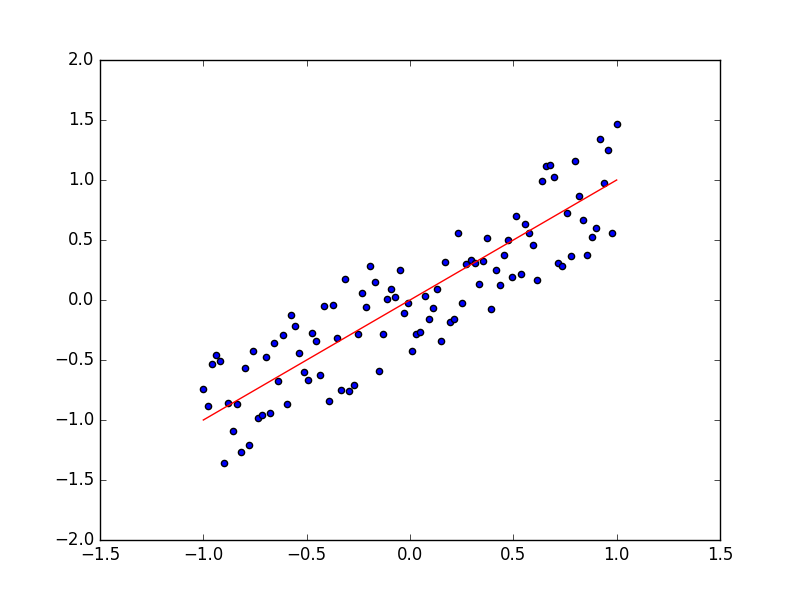
\includegraphics[scale=0.4]{linearNoise.png}
\end{figure}
Using Equation (1) with the values of $\theta_{1}$ and $\theta_{2}$ defined in Equations (9) and (10), we obtain the following regression line (in green), which is reasonably close to the original line (in red).
\begin{figure}[H]
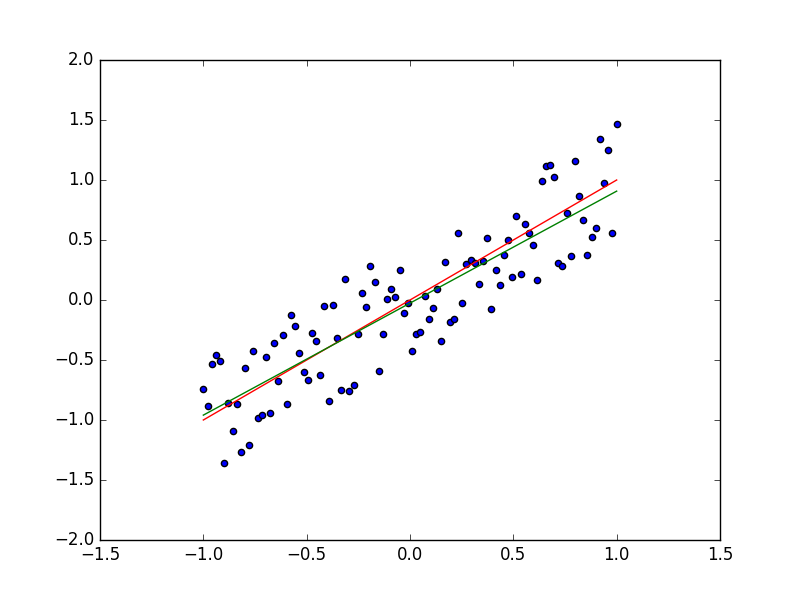
\includegraphics[scale=0.4]{linearNoiseWithRegression.png}
\end{figure}
\newpage
If we vary the value of $\theta_{1}$, the slope of the regression line changes, as illustrated below.
\begin{figure}[H]
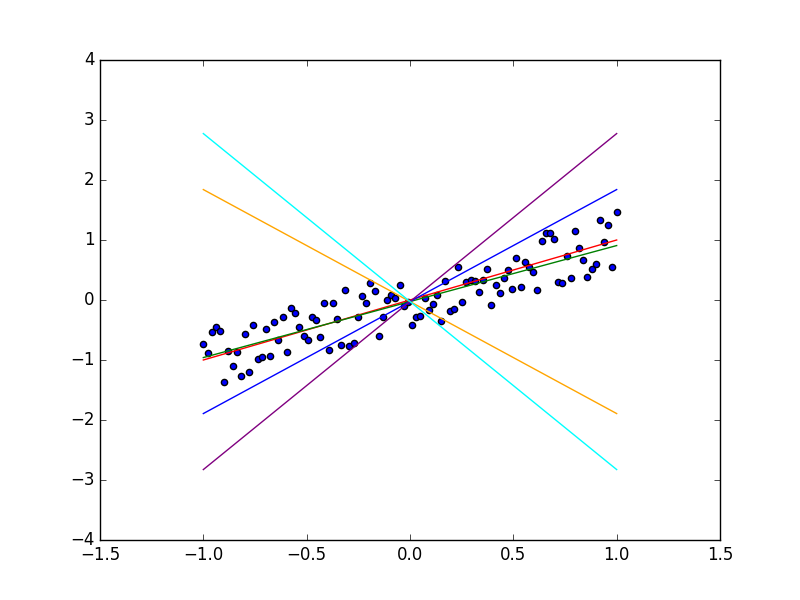
\includegraphics[scale=0.4]{linearNoiseVariationT1.png}
\end{figure}
If we vary the value of $\theta_{2}$, the regression line moves vertically in the x-y plane, as illustrated below.
\begin{figure}[H]
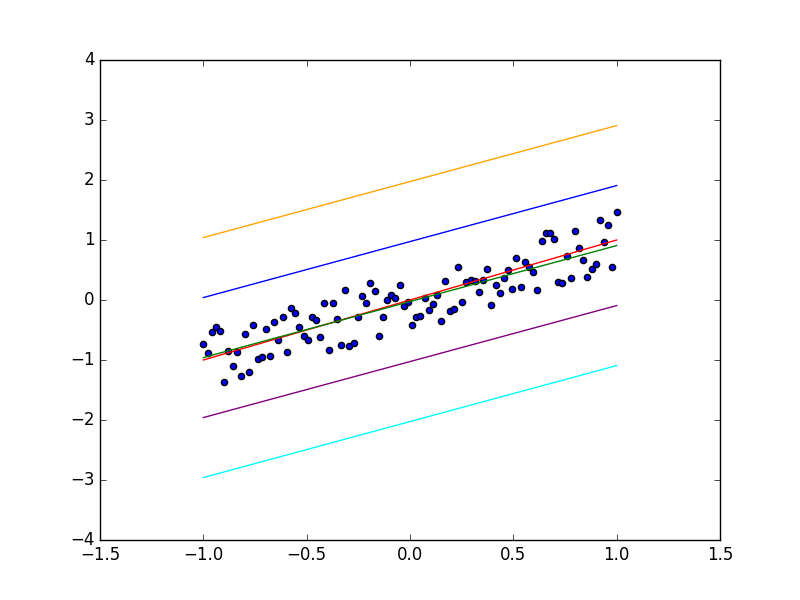
\includegraphics[scale=0.4]{linearNoiseVariationT2.png}
\end{figure}
\newpage
Now, we generate noisy data using the simple exponential function $y = e^x$ (shown in red).
\begin{figure}[H]
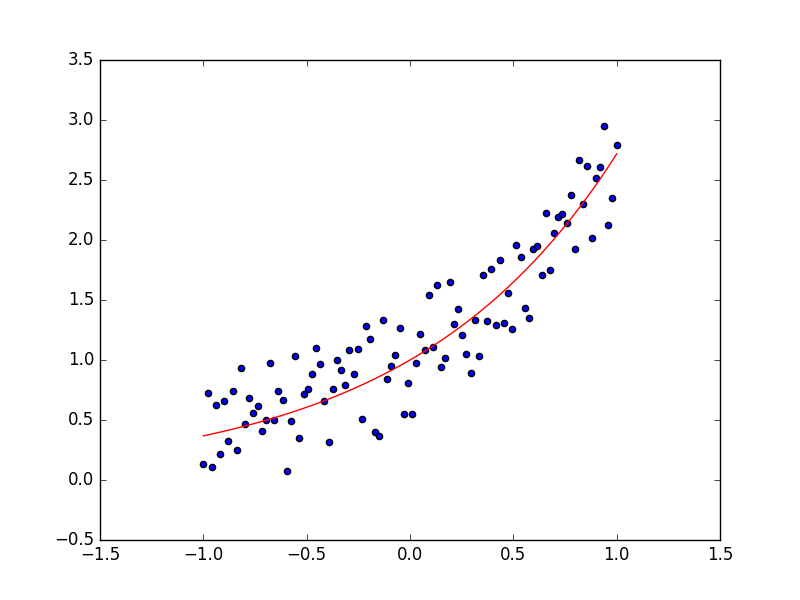
\includegraphics[scale=0.4]{expNoise.png}
\end{figure}
We must now change the functional form of the regression model from linear to exponential, as in Equation (12). Using the values of $\theta_{1}$ and $\theta_{2}$ from Equations (17) and (18), we obtain the following regression curve (shown in green)
\begin{figure}[H]
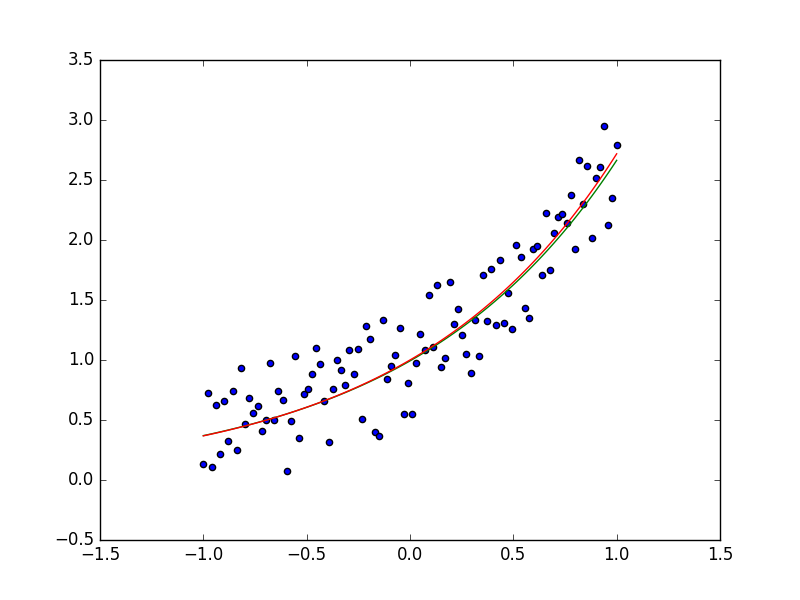
\includegraphics[scale=0.4]{expNoiseWithRegression.png}
\end{figure}
\newpage
Varying $\theta_{1}$, we obtain the following series of curves.
\begin{figure}[H]
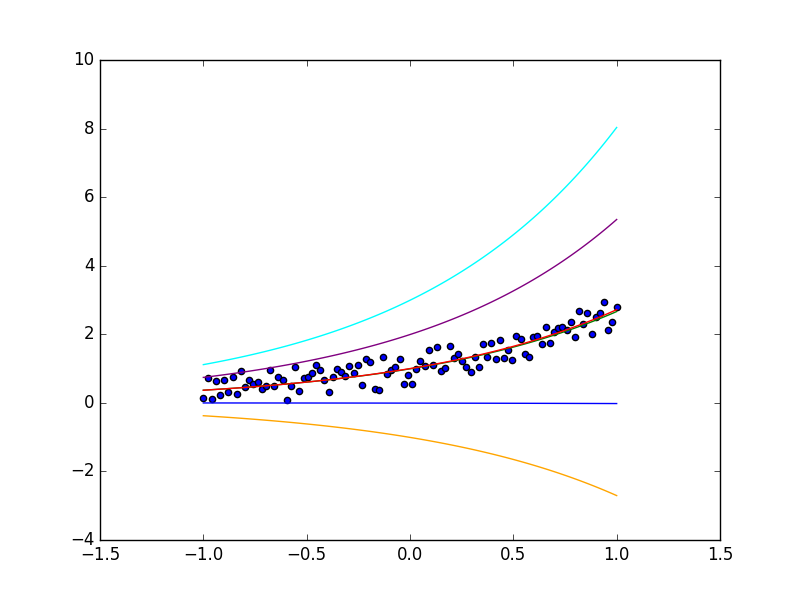
\includegraphics[scale=0.4]{expNoiseVariationT1.png}
\end{figure}
Similarly, varying $\theta_{2}$, we obtain the following:
\begin{figure}[H]
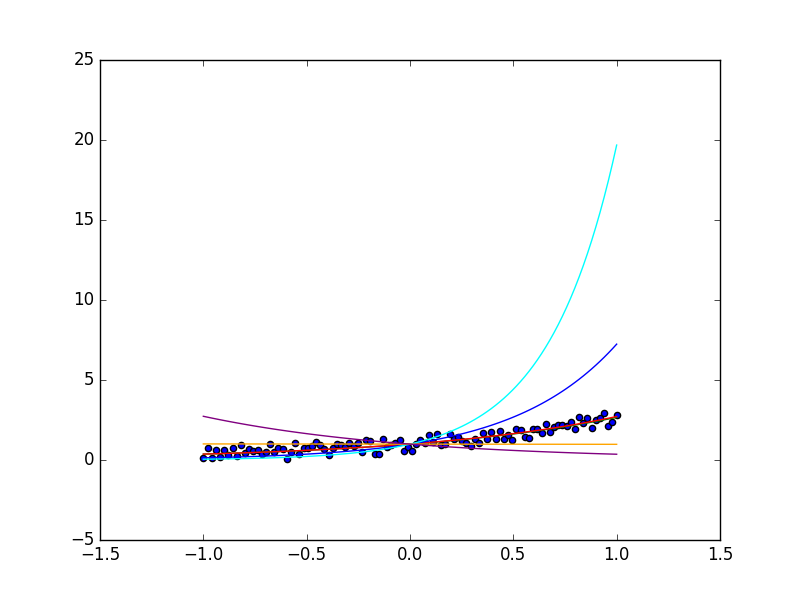
\includegraphics[scale=0.4]{expNoiseVariationT2.png}
\end{figure}
\newpage
\section{Optimization: Iterative Approach}
2.1\\
When a problem is impossible (or merely impractical) to optimize analytically, we can still optimize it numerically using iterative methods.\\
\\
a)\\
For continuous functions, gradients provide a useful optimisation approach as they show either the direction of descent (in the case of univariate functions) or the direction of steepest descent (in the case of multivariate functions).\\
\\
b)\\
We could evaluate sampled points across the domain of the function and then approximate the minimiser as the sampled point with the lowest function value. We could perhaps assign each sampled point a range to indicate the range around the point in which the minimiser could lie.\\
\\
2.2\\
\\
Let $f$ be a function in $\mathbf{R}$, let $x \in \mathbf{R}$ such that $f(x)=0$, and let $x_{0}$ be an approximation of $x$. The expansion of $f(x)$ as a Taylor series is
\begin{equation}
f(x) = f(x_{0})+(x-x_{0})f'(x_{0})+O((x-x_{0})^2)
\end{equation}
Thus, $f(x)$ approximates to
\begin{equation}
f(x) = 0 \approx f(x_{0})+(x-x_{0})f'(x_{0})
\end{equation}
which can be rearranged to
\begin{equation}
x \approx x_{0} - \frac{f(x_{0})}{f'(x_{0})} = x_{1}
\end{equation}
$x_{1}$ is a better approximation of $x$ than $x_{0}$. Repeating the process iteratively, we arrive at the Newton-Raphson method, which uses the formula
\begin{equation}
x_{k+1} = x_{k} - \frac{f(x_{k})}{f'(x_{k})}
\end{equation}
\newpage
a)\\
The Newton-Raphson can be used to optimise a function by finding the root of its derivative ($x$ such that $f'(x)=0$), which is necessary in order to minimise the error of the model.\\
\\
b)\\
In a machine learning context, $x_{i}$ can be interpreted as input data, $f(x_{i})$ as the class of $x_{i}$, and $f'(x_{i})$ as the rate at which the class changes with respect to the input data. The exact interpretations depend on the problem at hand.\\
\\
2.3\\
\\
Let $\bar{f}: \mathbf{R}^n \to \mathbf{R}^n$ and let $\bar{x} \in \mathbf{R}^n$. The expansion of $\bar{f}(\bar{x})$ as a Taylor series is
\begin{equation}
\bar{f}_{i}(\bar{x}+h\bar{x})=\bar{f}_{i}(\bar{x})+\sum\limits_{j=1}^n \frac{\partial \bar{f}_{i}(\bar{x})}{\partial x_{j}} h x_{j} + O(h \bar{x}^2) \approx \bar{f}_{i}(\bar{x})+\sum\limits_{j=1}^n \frac{\partial \bar{f}_{i}(\bar{x})}{\partial x_{j}} h x_{j}
\end{equation}
for each $i=1,...,n$. The n equations can be combined into a single equation
\begin{equation}
\bar{f}_{i}(\bar{x}+h\bar{x})\approx 
\begin{bmatrix}
f_{1}(\bar{x})\\
\vdots\\
f_{n}(\bar{x})
\end{bmatrix}
+
\begin{bmatrix}
\frac{\partial f_{1}}{\partial x_{1}} \dots \frac{\partial f_{1}}{\partial x_{n}}\\
\vdots \ddots \vdots\\
\frac{\partial f_{n}}{\partial x_{1}} \dots \frac{\partial f_{n}}{\partial x_{n}}
\end{bmatrix}
\begin{bmatrix}
h x_{1}\\
\vdots\\
h x_{n}
\end{bmatrix}
\end{equation}
which is simply
\begin{equation}
\bar{f}_{i}(\bar{x}+h\bar{x})\approx \bar{f}(\bar{x}) + J(\bar{x})h\bar{x}
\end{equation}
where $J$ denotes the Jacobian of $\bar{f}$. Setting Equation (25) equal to 0, we can solve for $h \bar{x}$, obtaining
\begin{equation}
h \bar{x} = J(\bar{x})^{-1}[\bar{f}(\bar{x}+h\bar{x})-\bar{f}(\bar{x})]=-J(\bar{x})^{-1}\bar{f}(\bar{x})
\end{equation} 
Thus, we can approximate the root as
\begin{equation}
\bar{x}+h\bar{x} = \bar{x}-J(\bar{x})^{-1}\bar{f}(\bar{x})
\end{equation}
As this is only an approximation of the root, we can improve our approximation by repeating the process iteratively, providing us with the formula for the n-dimensional Newton-Raphson method,
\begin{equation}
\bar{x}_{k+1} = \bar{x}_{k}-J(\bar{x}_{k})^{-1}\bar{f}(\bar{x}_{k})
\end{equation}
\newpage
2.4\\
The following python script implements the multivariate Newton-Raphson method described in 2.3.\\
\begin{lstlisting}
import numpy as np

def f(x):
    return np.array([[x.item(1) - x.item(0)**2],
                     [x.item(0)**2 + x.item(1)**2 - 1]
                     ], float)

def jacobian(x):
    return np.array([
                       [-2*x.item(0), 1],
                       [2*x.item(0), 2*x.item(1)]
                       ], float)

def newtonRaphson(x0,f,J,tol):
    x1 = x0 - np.matmul(np.linalg.inv(J(x0)), f(x0))
    while(np.all(x1-x0)>tol):
        x0 = x1
        x1 = x0 - np.matmul(np.linalg.inv(J(x0)), f(x0))
    return x1

x0 = np.array([[1],
              [1]
               ])
tol = 0.005
xroot = newtonRaphson(x0,f,jacobian,tol)
print(xroot)
\end{lstlisting}
The function \textit{newtonRaphson} actually implements the method, while the functions \textit{f} and \textit{jacobian} define an example function and its Jacobian. In this case, these were
\begin{equation}
\bar{f}(\bar{x}) = \begin{bmatrix}
x_{2}-x_{1}^2\\
x_{1}^2 + x_{2}^2 - 1
\end{bmatrix}, J(\bar{x}) = \begin{bmatrix}
-2 x_{1} & 1\\
2 x_{1} & 2 x_{2}
\end{bmatrix}
\end{equation}
The inputs seen in in the code ($x_{0} = [1,1]$ and $tol = 0.005$) give a final answer of $[0.78615138,0.61803399]$, which is correct within the tolerance.
\newpage
2.5\\
\\
One aspect for which we can test is how much time the algorithm takes given a problem of dimension $n$.\\
\\
To time the algorithm, a function and $x_{0}$ of dimension $n$ and a Jacobian of dimension $n \times n$  were supplied. The method was timed for 100 runs, and then this was repeated 100 times to produce the mean time it takes for the method to run 100 times for dimension $n$. The results are shown below for $n = 2,3,4,5,6$.
\begin{figure}[H]
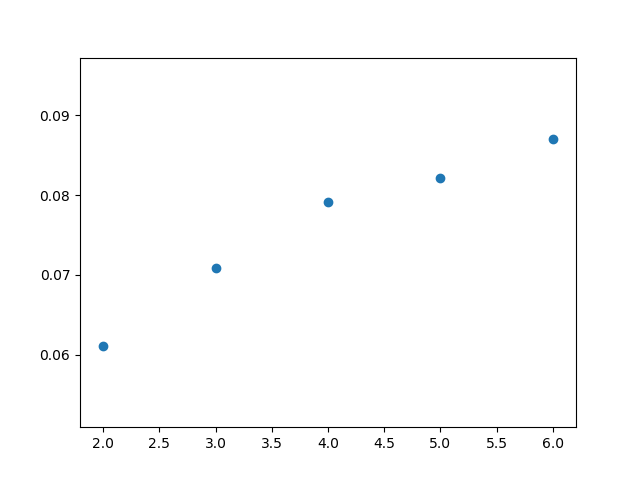
\includegraphics[scale=0.4]{newtonRaphsonPerformanceNvsTime.png}
\end{figure}
Applying a linear regression on the data, we arrive at the following graph
\begin{figure}[H]
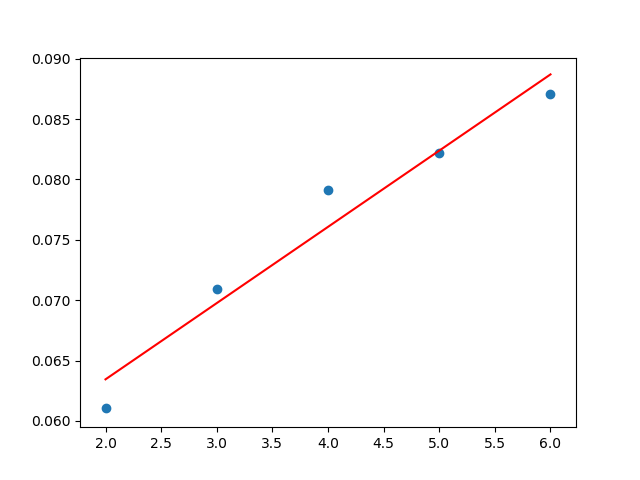
\includegraphics[scale=0.4]{newtonRaphsonPerformanceNvsTimeWithRegression.png}
\end{figure}
which displays the line $time = 0.0063128951 n + 0.0508223819$ seconds. Since the regression line fits the data reasonably well, we can assume that the time the algorithm takes to run will increase linearly as $n$ increases, which means we can expect the algorithm to run fairly well for large $n$.
\newpage
Another aspect for which we can test is the number of iterations it takes to find the root from an initial point a given distance away from the root.\\
\\
The method was run using initial points of increasingly greater distance from the actual root. In this case, this was repeated 10,000 times, with the initial point increasing by 10 each time. The graph below plots this distance against the number of iterations it took for the method to find the root.
\begin{figure}[H]
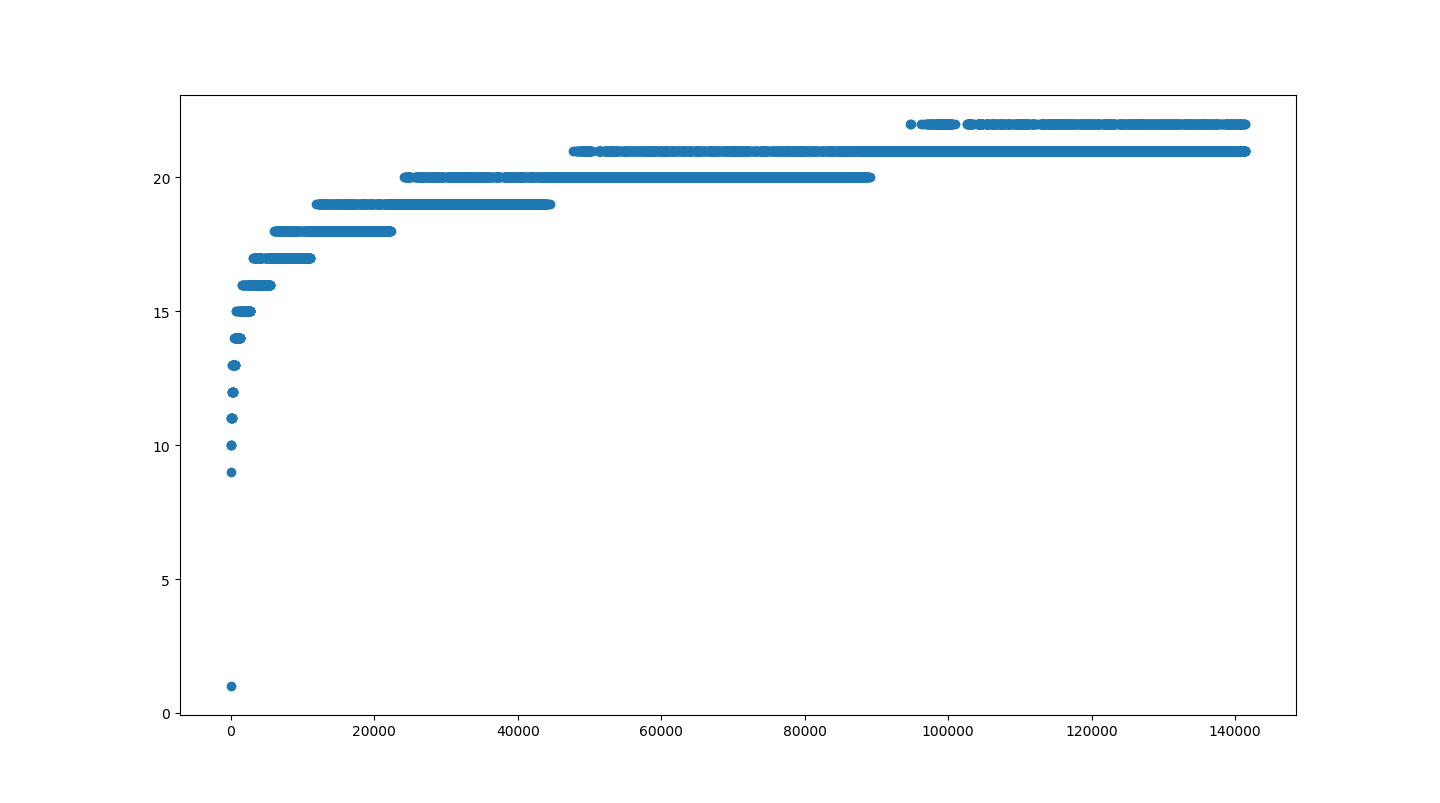
\includegraphics[scale=0.4]{newtonRaphsonPerformanceDistvsIters.png}
\end{figure}
The number of iterations plateaus as the distance increases, indicating that the method will find the root reasonably quickly from points a great distance away from it, provided there aren't other roots between the initial point and the desired root.\\
\\
Overall, it seems the Newton-Raphson method is robust enough to cope with problems of a large dimension and with initial approximations of incredibly poor accuracy (provided that there isn't much happening between the desired root and the initial point).
\newpage
2.6\\
a)\\
One could improve the Newton-Raphson method by changing it from the form given in Equation (28) to
\begin{equation}
\bar{x}_{k+1} = \bar{x}_{k}-\rho_{k} J(\bar{x}_{k})^{-1}\bar{f}(\bar{x}_{k}) 
\end{equation}
 This does introduce the problem of choosing a suitable $\rho_{k}$ for each iteration that improves convergence rather than hindering it.\\
 \\
 One downside of the Newton-Raphson method is that computing the inverse Jacobian each iteration can be prohibitively expensive and slow. We might be able to improve convergence by only updating the Jacobian every $\sigma$ iterations. This does introduce the problem of how to set the value of $\sigma$.\\
 \\
 b)\\
 If the function has many roots and a poor initial point is chosen, the method may converge to an undesired root (for example, a root which falls outside the desired parameter range) or, worse, may not converge at all (for example, an $x_{k}$ is chosen such that $x_{k+1} = x_{k}$). To overcome this, it is usually sufficient to choose an initial point close to the root.\\
\\
c)\\
If the function is "very wrinkly", the method would likely converge to an undesired root (for example, a very "shallow" optimum). The method can converge to undesired roots that are close to or far away from the initial point, and thus this problem can only be overcome with very careful selection of the initial point.
\end{document}